\documentclass[../main.tex]{subfiles}


\begin{document}

\section{Analyse}

%Indledning af analyse-afsnittet
\begin{flushleft} 
Intro tekst
\end{flushleft}


%Aktør
\subsection{Aktør}
Brætspillet indeholder én primær aktør:
\begin{itemize}
  \item  Spiller \\
\end{itemize}


%Use Case Diagram
\subsection{Use Case Diagram}
\begin{figure}[H]
    \centering
    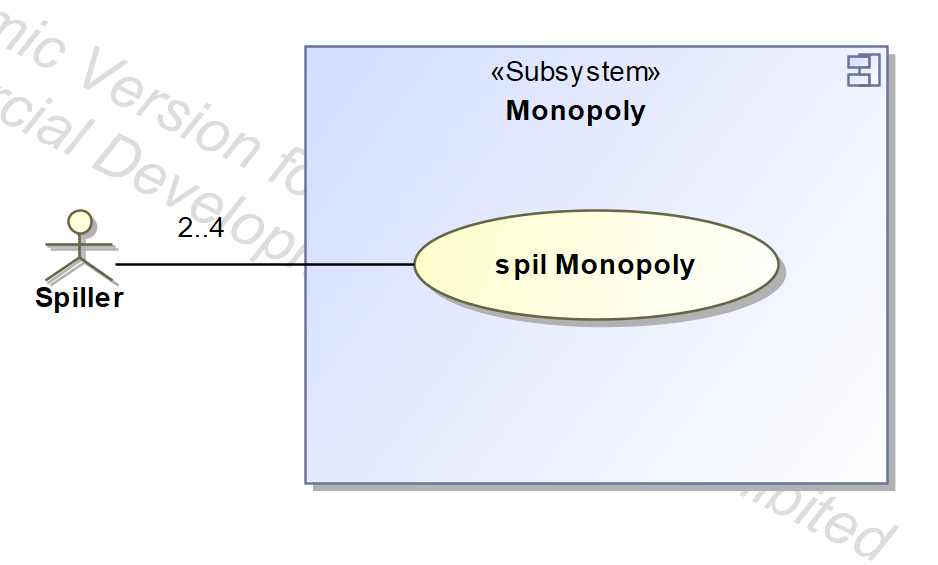
\includegraphics[width=0.6\linewidth]{figures/use-case_Diagram.png}
    \caption{Use-Case Diagram}
    \label{fig:UCDia}
\end{figure}

\newpage 

%Use Case tabel?
%ID, funktion, casual beskrivelse
\subsection{?Use Case tabeloversigt?}
\TODO[Skal dette evt. laves?]
\begin{figure}[H]
    \centering
    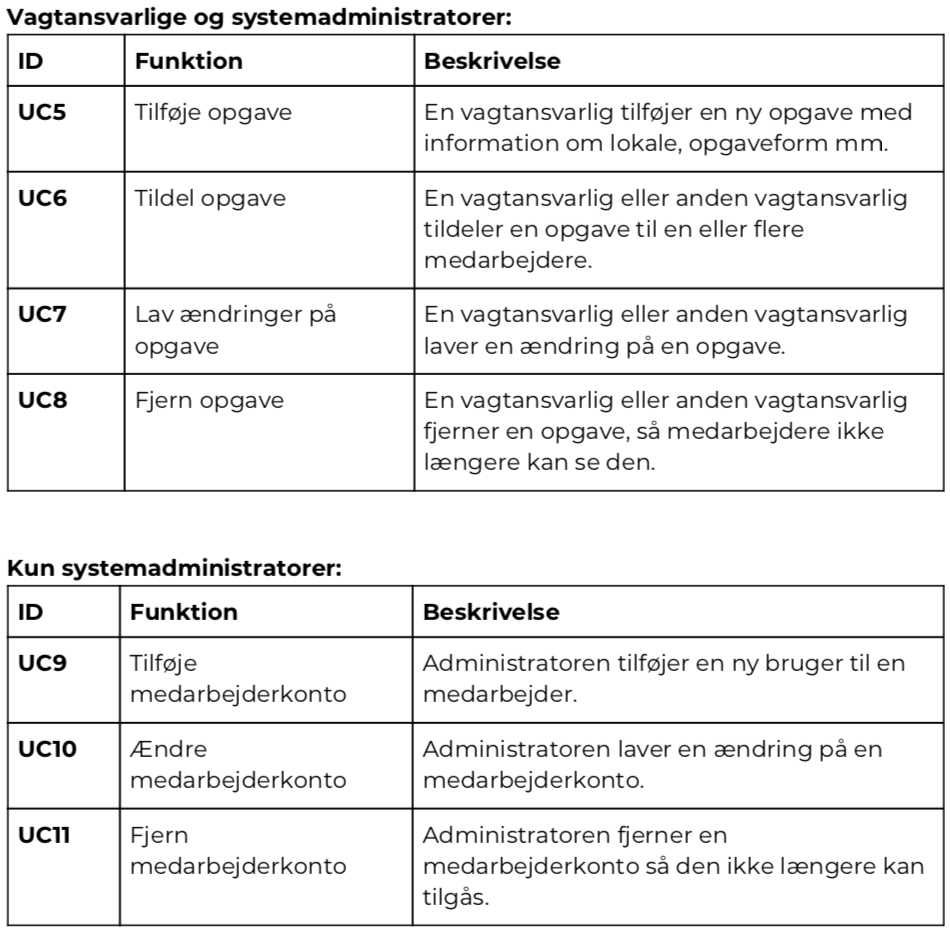
\includegraphics[width=0.6\linewidth]{figures/use-case-tabel-portalen.png}
    \caption{Use-Case Diagram}
    \label{fig:UCDia}
\end{figure}


%Use cases og tilhørende beskrivelser
\subsection{Use Cases og beskrivelser\textit{}}
\TODO[]
\begin{flushleft}Detaljeret use-case beskrivelse:\end{flushleft}

\begin{flushleft}Brief use-case beskrivelse:\end{flushleft}


% Domænemodel
\subsection{Domænemodel}
\begin{figure}[H]
    \centering
    \includegraphics[width=0.7\linewidth]{figures/domæne-model.png}
    \caption{Domænemodel til spillet}
    \label{fig:domain}
\end{figure}


% Systemsekvensdiagram
\subsection{Systemsekvensdiagram}
\TODO[]
\begin{figure}[H]
    \centering
    \includegraphics[width=0.7\linewidth]{figures/}
    \caption{Systemsekvensdiagram}
    \label{fig:systemsekvens}
\end{figure}



\end{document}